This section lists and explains basic layers used by neural networks described in this paper.
\subsection{Pooling}
A pooling function replaces the output at a certain location with a
summary statistic of the nearby outputs. \autocite{Goodfellow.2016} The following pooling functions are used by neural networks described in this paper.
\begin{itemize}
	\item Max Pooling
	\item Average Pooling
	\item Global Average Pooling
\end{itemize}
\subsubsection{Max Pooling}
The most widely used pooling technique is max pooling. Max pooling takes a maximum from all pools of input channels of the layer's input.\autocite{Singh.2020} The pools can be seen as array slices. These array slices are determined by pooling size $p$ and stride $stride$. The pooling size determines the shape of the pool. The pool is shaped $p \times p$. Stride is the number of rows and columns by which the pool is shifted to determine the next pool. This shifting can be imagined as sliding the pool over the input channel. Given an input channel $X$ with size $w \times h$, max pooling $maxpooling$ is defined as described by Equation \eqref{eq:pooling}. \autocite{Michelucci.2019}
\begin{equation}
	\label{eq:pooling}
	\begin{array}{l}
	maxpooling = max(X[i:i+p, j:j+p]) |\\
	i \in \{x|x_0=0, x \le w-p, x_{n+1} = x_n+stride\},\\
	j \in \{x|x_0=0, x \le h-p, _{n+1} = x_n+stride\}
	\end{array}
\end{equation}
For a better understanding, an example of max pooling is illustrated in Figure \ref{fig:pooling}. The figure displays an example of max pooling an input channel of shape $4 \times 4$, with a stride of 2, and a pooling size of 2. The different pools are highlighted in different colors. The result of a pool is highlighted in the color of that pool.
\begin{figure}[H]
	\centering
	\begin{tikzpicture}
\matrix (mtr) [matrix of nodes,row sep=-\pgflinewidth, nodes={draw}]
{
	|[fill=orange!30]| 8 & |[fill=orange!30]| 2 & |[fill=green!30!black!30]| 5 & |[fill=green!30!black!30]| 4 \\
	|[fill=orange!30]| 1 & |[fill=orange!30]| 0 & |[fill=green!30!black!30]| 7 & |[fill=green!30!black!30]| 1 \\
	|[fill=blue!30]| 1 & |[fill=blue!30]| 2 & |[fill=yellow!30]| 3 & |[fill=yellow!30]| 0 \\
	|[fill=blue!30]| 0 & |[fill=blue!30]| 2 & |[fill=yellow!30]| 1 & |[fill=yellow!30]| 2 \\ 
};

\node [below= of mtr-2-3.south west] (lm) {Input Channel};

\matrix (mt) [matrix of nodes,row sep=-\pgflinewidth, nodes={draw}, right = 4em of mtr]
{
	 |[fill=orange!30]| 8 &  |[fill=green!30!black!30]| 7 \\
	 |[fill=blue!30]| 2 &  |[fill=yellow!30]| 3 \\
};

\node [below= of mt-1-2.south west] (m) {Output};

\end{tikzpicture}
	\caption{Max Pooling Illustration (own figure)}
	\label{fig:pooling}
\end{figure}
\subsubsection{Average Pooling}
Another pooling technique is average pooling. 
%
Average pooling is used by DenseNet-264\autocite{Huang.2017} which is described in this paper. 
%
Understanding this neural network requires understanding average pooling. Average pooling works exactly the same as max pooling except that it takes the average instead of the maximum. Given an input channel~$X$ with size $w \times h$, average pooling~$avgpooling$ is defined as described by Equation~\eqref{eq:avgpooling}. \autocite{Michelucci.2019}
\begin{equation}
	\label{eq:avgpooling}
	\begin{array}{lcl}
		avgpooling & = & average(X[i:i+p, j:j+p]) |\\
		average(X) & = & \frac{\sum X}{|X|} 
	\end{array}
\end{equation}
\subsubsection{Global Average Pooling}
Another pooling technique is global average pooling. 
%
Global average pooling is used by ResNet-152\autocite{He.2016}, ResNeXt-101\autocite{Xie.2017}, DenseNet-264\autocite{Huang.2017}, and EfficientNet-B7\autocite{Tan.2019} which are described in this paper.
%
Understanding these neural networks requires understanding global average pooling. Global average pooling takes the average of each input channel. The input is an array of input channels. The output is an array containing the averages. Given an array of $d$ input channels $X$, global average pooling $globalavgpooling$ is defined as described by Equation \eqref{eq:globalavgpool}. \autocite{Lin.2013}
\begin{equation}
	\label{eq:globalavgpool}
	\begin{array}{lcl}
		globalavgpooling(X) & = & concat(globalavgpooling_0, \dots, globalavgpooling_{d-1})\\
		globalavgpoolingg_i & = & average(X_i)\\
		average(X) & = & \frac{\sum X}{|X|} 
	\end{array}
\end{equation}
 

\subsection{Dense}
A dense layer is a layer in which each neuron is connected to each input of the layer, see Figure \ref{fig:dense}. Given the weights of the neurons $W$, an input $X$, and an activation function $\varphi$, the dense layer $dense$ is described by Equation \eqref{eq:dense}. \autocite{Singh.2020}
\begin{equation}
	\label{eq:dense}
	dense(X) = \varphi(X \cdot W)
\end{equation}
\begin{figure}[H]
	\centering
	Dense convolutional neural networks address a problem of deep \ac{CNN}s. \autocite{Huang.2017}
\blockquote[\cite{Huang.2017}]{As information about the input or gradient passes through many layers, it can vanish and \enquote{washout} by the time it reaches the end (or beginning) of the network.
}
Dense convolutional neural networks address this problem by connecting all layers with each other, see Figure \ref{fig:denseconv}. The input of a layer is the concatenation of the original input and all outputs of previous layers. This way, information flow between layers in the network is encouraged. \autocite{Huang.2017}
\begin{figure}[H]
	\centering
	
%\cube{x offset}{y offset}{width}{height}{depth}{color}{fillcolor}
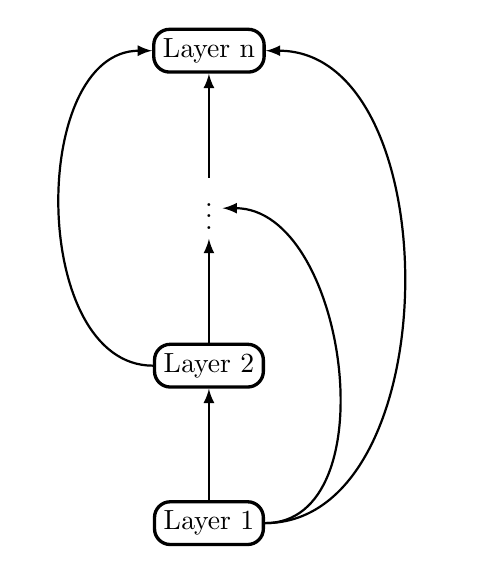
\begin{tikzpicture}[
	cell/.style={
		rectangle, 
		rounded corners=2mm, 
		draw,
		very thick,
		align=center,
	},
	ArrowC1/.style={% Arrows with rounded corners
		rounded corners=.25cm,
		thick,
	},
]

\node[cell] (l1) at (0,0) {Layer 1};
\node[cell] (l2) at (0,2) {Layer 2};
\node (dots) at (0,4) {$\vdots$};
\node[cell] (ln) at (0,6) {Layer n};

\draw[-latex, ArrowC1] (l1) -- (l2);
\draw[-latex, ArrowC1] (l2) -- (dots);
\draw[-latex, ArrowC1] (dots) -- (ln);

\draw[-latex, ArrowC1] (l1) to[out=0, in=0] (ln);
\draw[-latex, ArrowC1] (l1) to[out=0, in=0] (dots);

\draw[-latex, ArrowC1] (l2) to[out=-180, in=180] (ln);

	
\end{tikzpicture}
	\caption{Dense Convolutional Neural Network (own figure)}
	\label{fig:denseconv}
\end{figure}
\par
An additional, counter-intuitive effect of dense convolutional neural networks is that they require fewer parameters. 
Traditional neural networks pass information from layer to layer. Consequently, layers need to learn what information needs to be added and preserved. Dense convolutional neural networks explicitly distinguish between added and preserved information. Features are reused. Thus, they do not need to learn which information to preserve. Therefore, they need fewer parameters. \autocite{Huang.2017}
\par
The best-performing dense convolutional neural network found in the course of the literature review is the $264$ layer version of \cite{Huang.2017}'s DenseNet, called DenseNet-264.
The input of DenseNet-264 is a $224$-by-$224$-pixel, \ac{RGB} image. The output of DenseNet-264 comprises the probabilities of the $c$ target classes. 
DenseNet-264 is comprised of convolutional layers followed by $1$ dense layer. \autocite{Huang.2017}
\par
The convolutional layers have a stride of $1$ and a padding preserving spatial dimensions.
The first convolutional layer has $64$ kernels of size $7$ and a stride of $2$. It is followed by batch normalization, \ac{ReLU} activation function, and max pooling. Max pooling is applied with a pooling size of $3$, a pooling stride of $2$, and a padding preserving spatial dimensions. \autocite{Xie.2017}
The remaining convolutional layers are arranged in $4$ dense blocks and $3$ transition layers. A transition layer is applied between each dense block.
After the last dense block batch normalization, \ac{ReLU} activation function, global average pooling, and a dense layer are applied.
The dense layer has $c$ neurons and uses the softmax activation function. \autocite{Huang.2017}
\par
A dense block consists of $L$ convolutional blocks. All convolutional blocks are connected with each other. In consequence, the input of the $l$th convolutional block is the concatenation of the input of the dense block and the outputs of all previous layers. The output of the dense block is the concatenation of the input of the dense block and the outputs of all convolutional blocks of the dense block. Therefore, inside the dense block, the spatial dimensions of all feature maps are the same. A convolutional block consists of $2$~convolutional layers. The first layer has $128$~kernels of size~$1$. The second layer has $32$~kernels of size~$3$. Batch normalization and \ac{ReLU} activation function are applied before each convolution. The configurations of each dense block are outlined in Table \ref{tab:densenet}. \autocite{Huang.2017}
\par
A transition layer reduces the number and spatial dimensions of the feature maps.
A transition layer consists of the sequence batch normalization, \ac{ReLU} activation function, convolution, and average pooling. The convolution is used to reduce the number of feature maps by factor $0.5$. Hence, the convolution has $0.5 \cdot d$ kernels of size~$1$ with $d$ being the initial number of feature maps. The average pooling is used to reduce the spatial dimensions of the feature maps. The pooling is of size $2$ and has a stride~of~$2$. \autocite{Huang.2017}
\par
The whole configuration of DenseNet-264 is outlined in Table \ref{tab:densenet}. \autocite{Huang.2017}
\begin{xltabular}{\textwidth}{lX}\toprule
	\caption[DenseNet-264 Configuration]{DenseNet-264 Configuration. Note that each $k \times k \text{ conv } K$ denotes the sequence batch normalization, \ac{ReLU}, and convolution with $K$ kernels of size  $k$, except for the first $\text{conv}$, which denotes the sequence convolution, batch normalization \ac{ReLU}.} \label{tab:densenet}\\
	\textbf{Layer/Block} & \textbf{Configuration}\\\midrule \endhead
	Input Layer & $7 \times 7 \text{ conv } 64$, stride $2$, and $3 \times 3$ max pooling, stride $2$\\\midrule
	Dense Block $1$ & $\begin{bmatrix}
	1 \times 1 \text{ conv } 128\\
	3 \times 3 \text{ conv } 32
	\end{bmatrix} \times 6$\\\midrule
	Transition Layer $1$ & $1 \times 1 \text{ conv } 0.5d$, stride $2$, and $2 \times 2$ average pooling, stride $2$\\\midrule
	Dense Block $2$ & $\begin{bmatrix}
	1 \times 1 \text{ conv } 128\\
	3 \times 3 \text{ conv } 32
	\end{bmatrix} \times 12$\\\midrule
	Transition Layer $2$ & $1 \times 1 \text{ conv } 0.5d$, stride $2$, and $2 \times 2$ average pooling, stride $2$\\\midrule
	Dense Block $3$ & $\begin{bmatrix}
	1 \times 1 \text{ conv } 128\\
	3 \times 3 \text{ conv } 32
	\end{bmatrix} \times 64$\\\midrule
	Transition Layer $3$ & $1 \times 1 \text{ conv } 0.5d$, stride $2$, and $2 \times 2$ average pooling, stride $2$\\\midrule
	Dense Block $4$ & $\begin{bmatrix}
	1 \times 1 \text{ conv } 128\\
	3 \times 3 \text{ conv } 32
	\end{bmatrix} \times 48$\\\midrule
	Output Layer & batch normalization, \ac{ReLU}, global average pooling, and dense with $c$ neurons
	\\\bottomrule
\end{xltabular}
	\caption{Dense Layer (own figure)}
	\label{fig:dense}
\end{figure}


\subsection{Batch Normalization}
Batch normalization is a technique to speed up training. Training is sped up by smoothing the optimization landscape and stabilizing the gradients. \autocite{Santurkar.2018}
Batch normali\-zation normalizes an input by subtracting the mean and dividing by the standard deviation. Mean and standard deviation are approximated batch-wise. Computation over a batch is more efficient, but mean and standard deviation vary dependent on the batch. Therefore, the true mean and standard deviation are approximated over multiple batches by learnable parameters. Given a batch of $m$ inputs $\mathcal{B} = \{x_1, x_2, \dots, x_m \}$, learnable parameters $\gamma, \beta$, and a noise $\epsilon$, batch normalization $batchnorm$ is defined by Equation \eqref{eq:batchnorm}. \autocite{Ioffe.2015} Noise ensures that division by $0$ does not occur.
\begin{equation}
	\label{eq:batchnorm}
	\begin{array}{lcl}
		batchnorm(x) & = & \gamma \hat{x} + \beta \\
		\hat{x} & = & \frac{x-\mu}{\sqrt{\sigma^2+\epsilon}}\\
		\mu & = & \frac{1}{m} \sum_{i=1}^{m} b_i | b_i \in \mathcal{B}\\
		\sigma & = & \frac{1}{m} \sum_{i=1}^{m} (b_i-\mu)^2 | b_i \in \mathcal{B}\\
	\end{array}
\end{equation}

\subsection{Dropout}
Dropout is a regularization technique addressing the problem of overfitting. 
Dropout randomly drops neurons during training. Dropping means removing the neuron temporarily, along with its connections. The probability of a neuron being dropped is called dropout rate $q$. Neurons are only dropped during training. After training, each neuron is retained and their weights are scaled down by the probability of a neuron being retained $p=1-q$.\autocite{Srivastava.2014}





%\subsection{Flatten} brauchst du nicht? Weil def dens layer alle neurons zu allen connected ist da ist egal ob vector oder matrix oder 3d tensor